%%%%%%%%% Notes %%%%%%%%%

%%%%%%%%% Packages %%%%%%%%%
\documentclass[aspectratio=43]{beamer}
\usepackage[T1]{fontenc}
\usepackage{derivative}
\usepackage{pgfpages}

%%%%%%%%% Packages setup %%%%%%%%%
\setbeameroption{show notes on second screen}
%\setbeameroption{show only notes}
%\setbeamerfont{note page}{size=\tiny}
\setbeamercolor{note page}{bg=white, fg=black}
\setbeamercolor{note title}{bg=white!99!black, fg=black}
\usetheme{Hannover}
\usecolortheme{spruce}
\graphicspath{{./figures/}{../code/figures/}}

%%%%%%%%% Macros %%%%%%%%%
\newcommand{\transpose}{\intercal}

%%%%%%%%% Document informations %%%%%%%%%
\title{Summary of \emph{A tutorial on the free-energy framework for modelling perception and learning} by Rafal Bogacz}
\author{Marco Casari}
\date[12/12/2023]{Complex system in neuroscience, 12 December 2023}
\institute[UniTo]{University of Turin}

%%%%%%%%% Document %%%%%%%%%
\begin{document}
\begin{frame}
  \titlepage
  \note{
    \begin{itemize}
      \item In this presentation the main topics of the paper are presented in order of appearance.
      % MC also write that my results from exercises are present if I decide to put them in the presentation.
    \end{itemize}
  }
\end{frame}



\section{Introduction}
\begin{frame}
  \frametitle{Introduction}
  \begin{itemize}
    \item<1-> Predictive coding model of Rao and Ballard.
    \note[item]<1->{Prior predictions are compared to stimuli and the model parameters are updated considering prediction errors, features corresponding to receptive fields in the the primary sensory cortex are learned.}
    \item<2-> Free-energy model of Friston.
    \note[item]<2->{Weight stimuli by their noise, learn features using their covariance, implement attentional modulation changing the variance of attended features.}
    \item<3-> Hebbian plasticity.
    \note[item]<3->{Synaptic strenght is changed proportionally to activities of pre-synaptic and post-synaptic neurons.}
    \item<4-> Free energy minimization.
    \note[item]<4->{Minimization of free energy can be seen as the base of many theories of perception.}
  \end{itemize}
\end{frame}

\begin{frame}
  \frametitle{Working hypotheses}
  \begin{enumerate}
    \item<1-> Local computation.
    \note[item]<1->{The state of a neuron is determined only by the synaptic weight and the state of its input neurons.}
    \item<2-> Local plasticity.
    \note[item]<2->{Synaptic plasticity depends only on the activities of pre-synaptic and post-synaptic neurons.}
    \item<3-> Basic neuronal computation.
    \note[item]<3->{The state of a neuron is the result of the application of a monotonic function to the linear combination of states and synaptic weights of input neurons.}
  \end{enumerate}
\end{frame}



\section{Single variable model}
\begin{frame}
  \frametitle{Single variable model}
  \begin{itemize}
    \item<1-> Feature is a scalar variable $v \in \Omega_v$.
    \item<1-> Stimulus is a scalar variable $u \in \Omega_u$.
    \note[item]<1->{The model describes the inference of a single variable from a single sensory input.}
    \item<2-> Relation between feature and stimulus is a differentiable function $g : \Omega_v \to \Omega_u$.
    \note[item]<2->{In general inferred variable and sensory input are related by some smooth function.}
    \item<3-> Sensory input $p(u | v)$ is affected by gaussian noise and it has mean $g(v)$ and variance $\Sigma_u$.
    \note[item]<3->{Sensory input and stimulus are drafted from the same space.}
    \item<4-> Prior knowledge of the feature $p(v)$ follows a gaussian distribution with mean $v_p$ and variance $\Sigma_p$.
    \note[item]<4->{Information gained and constantly updated from previous experience.}
  \end{itemize}
\end{frame}

\begin{frame}
  \frametitle{Exact solution to the inference problem}
  \begin{itemize}
    \item<1-> Bayes theorem:
      \begin{equation}
        \label{eq:bayes}
        p(v | u) = \frac{p(v) p(u | v)}{p(u)}
        \quad .
      \end{equation}
    \note[item]<1->{Knowledge of feature depending on a given stimulus is the posterior. Prior knowledge on the feature is the prior, distribution of stimulus is the likelihood.}
    \item<2-> Marginal likelihood of stimuli:
      \begin{equation}
        \label{eq:marginal}
        p(u) = \int_{\Omega_v} p(v) p(u | v) \odif{v}
        \quad .
      \end{equation}
    \note[item]<2->{In general, marginal likelihood is difficult to evaluate.}
    \item<3-> No implementation in simple biological systems.
    \note[item]<3->{Complex calculations and infinite nodes are needed to represent each value of the posterior.}
  \end{itemize}
\end{frame}

% MC insert Exercise_1.

\begin{frame}
  \frametitle{Approximate solution to the inference problem}
  \begin{itemize}
    \item<1-> Most likely value of the feature is a scalar variable $\phi \in \Omega_v$.
    \note[item]<1->{Evaluating the mode of the posterior instead of the whole function is more biologically plausible.}
    \item<2-> Equivalent to maximize negative free energy with respect to the feature:
      \begin{equation}
        \label{eq:negative_free_energy}
        F(v, u) = \ln{\big( p(v) p(u | v) \big)}
        \quad .
      \end{equation}
    \note[item]<2->{The most likely feature value is the fixed point of the gradient descent method applied to the negative free energy.}
    \item<3-> Prediction errors:
      \begin{align}
        \label{eq:error_prior}
        \varepsilon_p = \frac{v - v_p}{\Sigma_p}
        \quad , \\
        \label{eq:error_stimulus}
        \varepsilon_u = \frac{u - g(v)}{\Sigma_u}
        \quad .
      \end{align}
    \note[item]<3->{Prediction errors are introduced as new variables to extend the dynamical system and satisfy Hebbian plasticity.}
  \end{itemize}
\end{frame}

% MC insert Exercise_2.

\begin{frame}
  \frametitle{Neural implementation}
  \begin{center}
    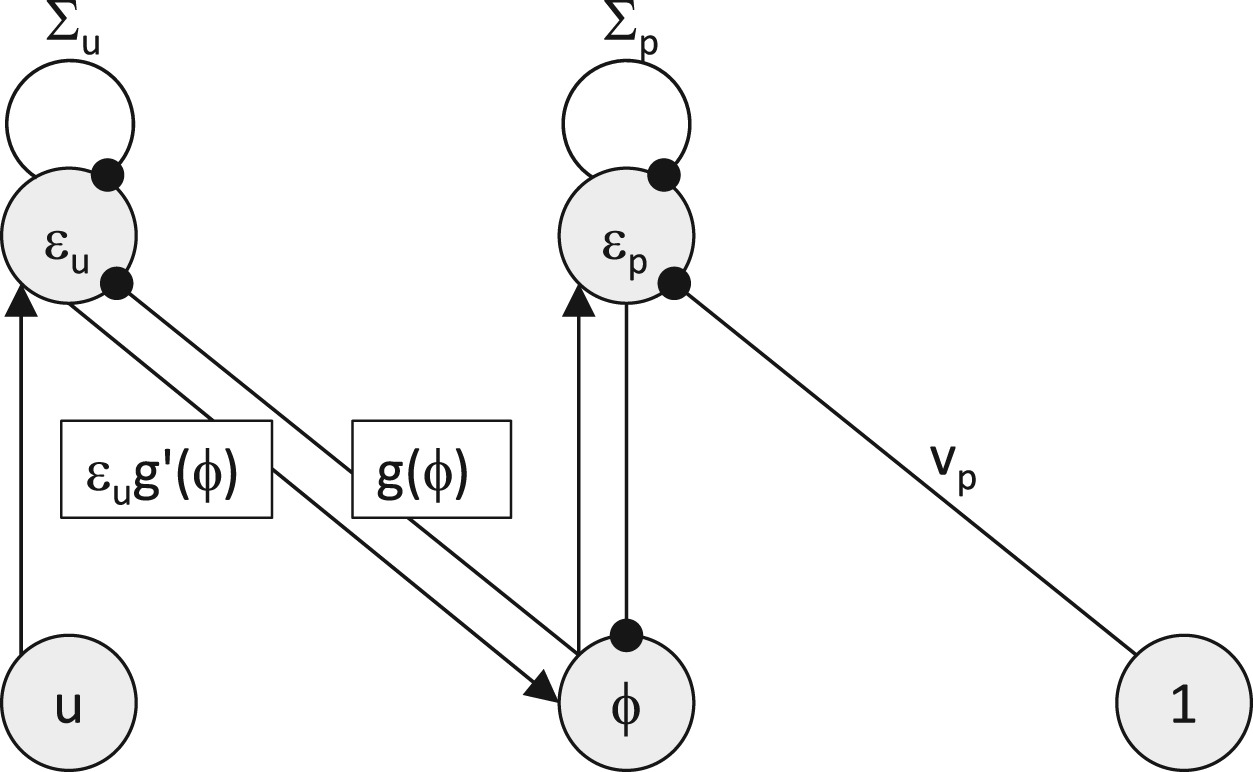
\includegraphics[width=0.5\textheight]{Fig3}
  \end{center}
  Fig. 3 from article: network implementation of the dynamical system
  \begin{equation}
    \label{eq:dynamical_system_single}
    \begin{cases}
      \dot{\phi} = \varepsilon_u g^\prime(\phi) - \varepsilon_p \\
      \dot{\varepsilon}_p = \phi - v_p - \Sigma_p \varepsilon_p \\
      \dot{\varepsilon}_u = u - g(\phi) - \Sigma_u \varepsilon_u
    \end{cases}
    \quad .
  \end{equation}
  \note{
    \begin{itemize}
      \item Note that hypotheses and Hebbian plasticity are satisfied.
    \end{itemize}
  }
\end{frame}

% MC insert Exercise_3.

\begin{frame}
  \frametitle{Learning model parameters}
  \begin{itemize}
    \item<1-> Choose model parameters to maximize $p(u)$.
    \note[item]<1->{Model parameters are mean and variance of variables.}
    \item<2-> Equivalent to maximize negative free energy with respect to parameters:
      \begin{align}
        \label{eq:gradient_mean_prior}
        \pdv{F}{v_p} & = \frac{\phi - v_p}{\Sigma_p}
        \quad , \\
        \label{eq:gradient_variance_prior}
        \pdv{F}{\Sigma_p} & = \frac{1}{2} \Bigg( \frac{(\phi - v_p)^2}{\Sigma_p^2} - \frac{1}{\Sigma_p} \Bigg)
        \quad , \\
        \label{eq:gradient_variance_stimulus}
        \pdv{F}{\Sigma_u} & = \frac{1}{2} \Bigg( \frac{(u - g(\phi))^2}{\Sigma_u^2} - \frac{1}{\Sigma_u} \Bigg)
        \quad .
      \end{align}
    \note[item]<2->{The fixed point of this dynamical system exists only as sample mean over the occured events of perception, where most likely feature value and stimulus are known.}
    \item<3-> Hebbian plasticity is satisfied using prediction errors.
    \note[item]<3->{Without prediction errors, the computation is still local.}
  \end{itemize}
\end{frame}

\begin{frame}
  \frametitle{Learning relation parameter}
  \begin{itemize}
    \item<1-> Linear relation:
      \begin{equation}
        \label{eq:relation_linear}
        g(v, \theta) = \theta v
        \quad .
      \end{equation}
    \note[item]<1->{Only one parameter is considered without loss of generality.}
    \item<2-> Nonlinear relation:
      \begin{equation}
        \label{eq:relation_nonlinear}
        g(v, \theta) = \theta h(v)
        \quad .
      \end{equation}
    \note[item]<2->{The nonlinearity increases the complexity of the network and partially changes Hebbian plasticity, still keeping it local.}
    \item<3-> Gradient of negative free energy for learning:
      \begin{equation}
        \label{eq:relation_nonlinear}
        \pdv{F}{\theta} = \frac{u - \theta h(\phi)}{\Sigma_u} h(\phi) = \varepsilon_u h(\phi)
        \quad .
      \end{equation}
    \note[item]<3->{Same consideration of model parameters apply to the relation parameter.}
  \end{itemize}
\end{frame}

\begin{frame}
  \frametitle{Free energy framework}
  \begin{itemize}
    \item<1-> Minimization of Kullback-Leibler divergence:
      \begin{equation}
        \label{eq:kl_divergence}
        KL(q(v) || p(v | u)) = \int_{\Omega_v} q(v) \ln \Bigg( \frac{q(v)}{p(v | u)} \Bigg) \odif{v}
        \quad .
      \end{equation}
    \note[item]<1->{In general, the posterior is approximated by a simpler probability distribution and the divergence between the two is minimized.}
    \item<2-> Definition of negative free energy:
    \begin{equation}
      \label{eq:negative_free_energy_definition}
      F(v, u) = \int_{\Omega_v} q(v) \ln \Bigg( \frac{p(v, u)}{q(v)} \Bigg) \odif{v}
      \quad .
    \end{equation}
    \note[item]<2->{Minimize KL divergence or maximize negative free energy to learn most likely model value, maximize marginal likelihood or maximize negative free energy to learn model parameters.}
    \item<3-> For the models discussed in the paper: $q(v) = \delta(v - \phi)$.
    \note[item]<3->{Equation~\eqref{eq:negative_free_energy} is recovered using delta function centered in the most likely feature value as probability distribution.}
  \end{itemize}
\end{frame}



\section{Multiple variables model}
\begin{frame}
  \frametitle{Multiple variables model}
  \begin{center}
    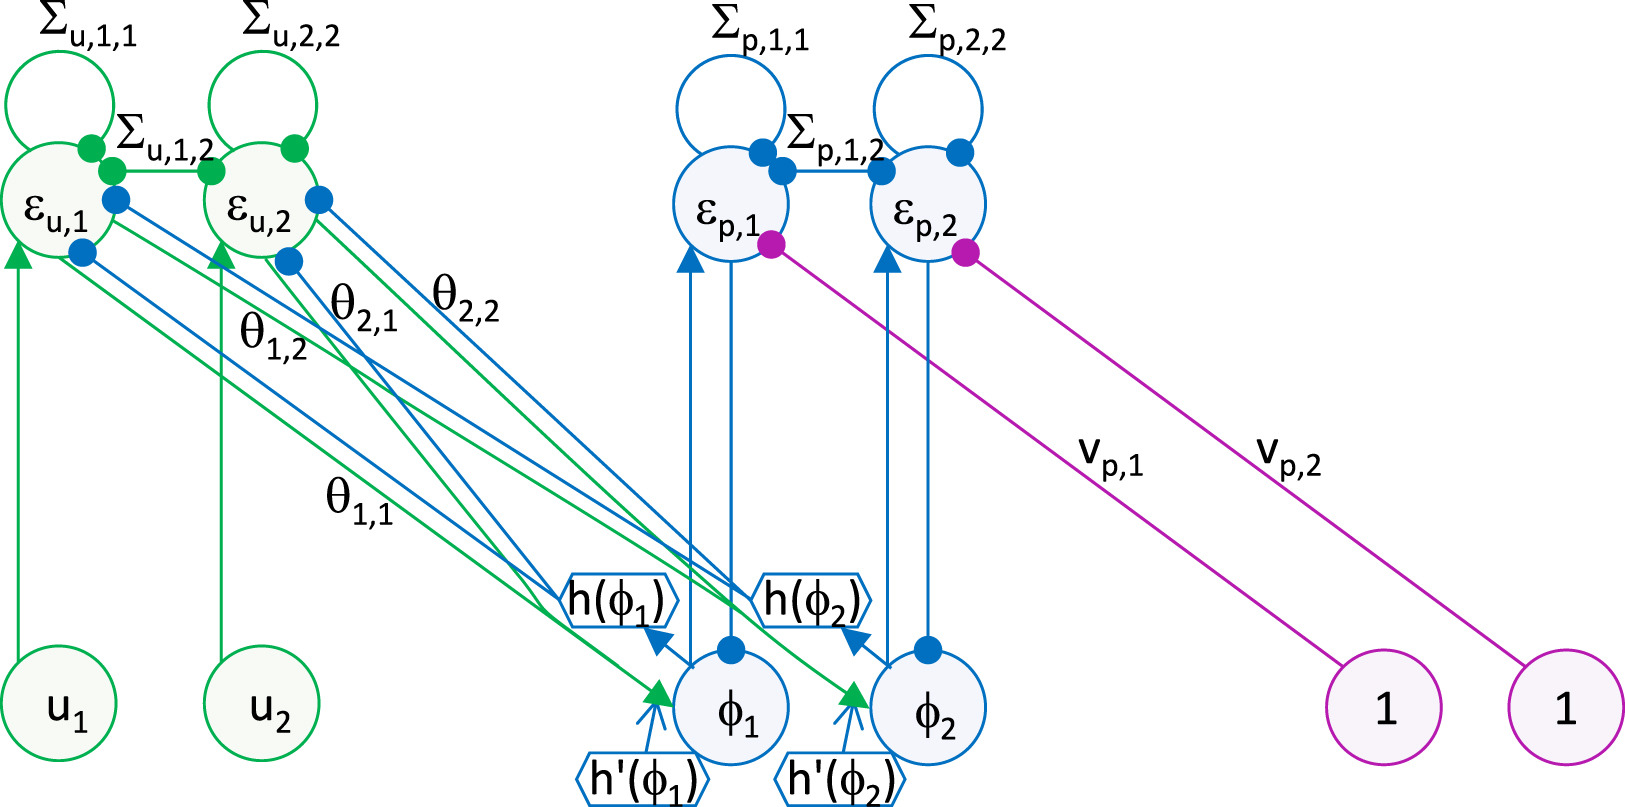
\includegraphics[width=0.8\textheight]{Fig5}
  \end{center}
  Fig. 5 from article: example of a model with 2 features and 2 stimuli. Equations are rewritten using matrix notation, but local plasticity is not satisfied.
  \note{
    \begin{itemize}
      \item Calculus rules are extended to work elementwise on vectors and matrices, multivariate gaussian distribution and nonlinear relation between variables and stimuli are used.
      \item The inverse of covariance matrix depends on non-adjacent neurons, Hebbian plasticity is again partially satisfied.
    \end{itemize}
  }
\end{frame}

\begin{frame}
  \frametitle{Hierarchical structure implementation}
  \begin{itemize}
    \item<1-> Parallel to structure of cortical areas.
    \note[item]<1->{Information is used and travels in different layers of the cortex.}
    \item<2-> Generalized equations for the inference task:
      \begin{align}
        \label{eq:dynamical_system_phi}
        \dot{\vec{\phi}}_i & = - \vec{\varepsilon}_i + h^\prime(\vec{\phi}_i) \times \boldsymbol{\Theta}_{i-1}^\transpose \vec{\varepsilon}_{i-1}
        \quad , \\
        \label{eq:dynamical_system_epsilon}
        \dot{\vec{\varepsilon}}_i & = \vec{\phi}_i - \boldsymbol{\Theta}_i h(\vec{\phi}_{i+1}) - \boldsymbol{\Sigma}_i \vec{\varepsilon}_i
        \quad .
      \end{align}
    \item<2-> Generalized equations for the learning task:
      \begin{align}
        \label{eq:dynamical_system_sigma}
        \pdv{F}{\boldsymbol{\Sigma}_i} & = \frac{1}{2} (\vec{\varepsilon}_i \vec{\varepsilon}_i^\transpose - \boldsymbol{\Sigma}_i^{-1})
        \quad , \\
        \label{eq:dynamical_system_theta}
        \pdv{F}{\boldsymbol{\Theta}_i} & = \vec{\varepsilon}_i h(\vec{\phi}_{i+1})^\transpose
        \quad .
      \end{align}
    \note[item]<2->{Note the elementwise product and matrices of model and relation parameters.}
  \end{itemize}
\end{frame}

\begin{frame}
  \frametitle{Recover local plasticity}
  \begin{center}
    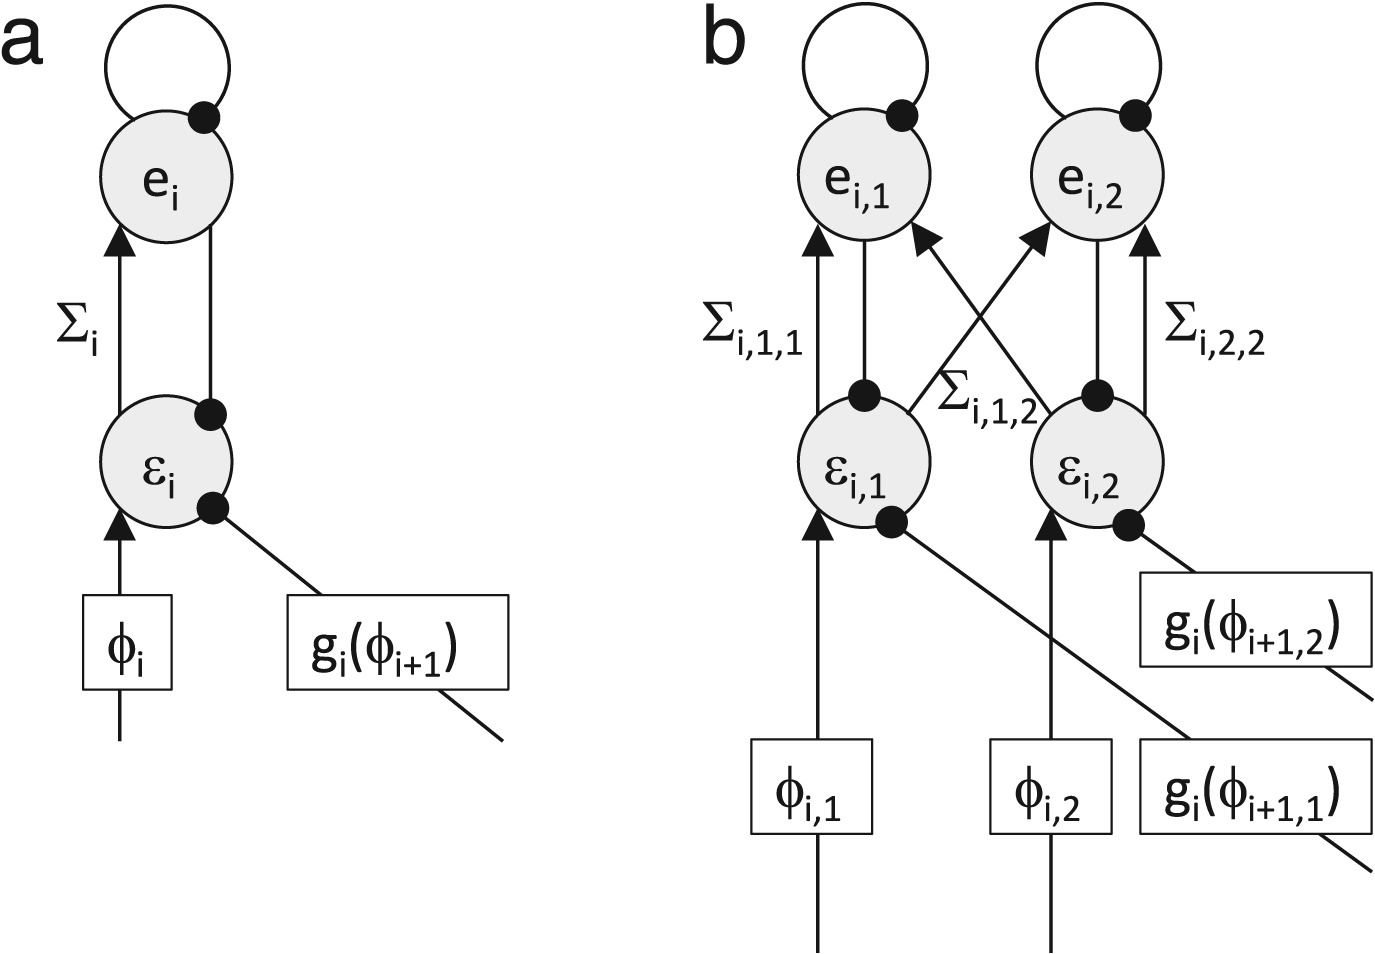
\includegraphics[width=0.4\textheight]{Fig7}
  \end{center}
  Fig. 7 from article: networks satisfying local plasticity for (a) single variable model and (b) multiple variables model. They implement the generalized dynamical system
  \begin{equation}
    \label{eq:dynamical_system_prediction_errors}
    \begin{cases}
      \dot{\vec{\varepsilon}}_i = \vec{\phi}_i - g_i(\vec{\phi}_{i+1}) - \vec{e}_i \\
      \dot{\vec{e}}_i = \boldsymbol{\Sigma}_i \vec{\varepsilon}_i - \vec{e}_i
    \end{cases}
    \quad .
  \end{equation}
  \note{
    \begin{itemize}
      \item The update rule for the model parameters is Hebbian and contains the learning rate as hyperparameter of the model.
      \item Convergence of prediction errors to the sample variances is guaranteed if the most likely feature values change at slower time scales.
    \end{itemize}
  }
\end{frame}

% MC insert Exercise_5.



\section{Conclusion}
\begin{frame}
  \frametitle{Conclusion}
  \begin{itemize}
    \item Stimuli weighted by noise.
    \item Learn covariance of stimuli.
    \item Attentional modulation.
  \end{itemize}
%  \vfill
%  \onslide<2->{
%    \centering
%    \huge
%    Thank you
%  }
\end{frame}
\end{document}
